\subsection{Kommunikationslänk}
Kommunikationslänken är uppdelad i två delar, USB kommunikation mellan routern och ADKn 
samt blåtandskommunikation mellan routern och fjärrkontrollen. Kommunikationen sker med hjälp av ett protokoll som 
togs fram under projektets gång. De tre första bitarna som skickas innehåller information om vart meddelandet ska skickas, 
vilken slags meddelande det är samt meddelandets längd. Utöver dessa tre bitar skickas datapaketet som konstruerats enligt 
Protocol Buffer som beskrivs i avsnitt \ref{komlank:ProtocolBuffer}. I figur \ref{fig:protocol} ses en grafisk illustarion av protokollet.


\begin{figure}[htbp!]
\centering
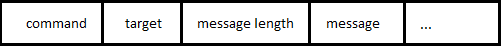
\includegraphics[width=10cm]{../../includes/figures/protocol.png}
\caption{Illustering av protokoll.}
\label{fig:protocol}
\end{figure}

\subsubsection{USB-kommunikation}
USB-kommunikationen mellan ADK:n och routern sker över Android Open Accessory (AOA) protokollet. 
För att få USB-kommunikationen att fungera användes Arduinos färdiga bibliotek [\ldots][VAD SKA REFEREAS TILL?]. En funktion i biblioteket justerades för 
att lösa ett initieringsfel. Se Wiki på podio.
 
Fördelen med detta bibliotek är att den implementerar AOA och tillhandahåller enkla funktioner för att läsa och skriva via USB, vilket 
gjorde det enklare att implementera det egendesignade protokollet.

I Android är implementationen av AOA och det egendesignade protokollet mer komplicerat. Den kod som hanterar USB-kommunikationen ligger 
i klassen UsbService. I denna klass får applikationen tillgång till Blåtandsadaptern och inititerar kommunikationen med ADK:n. 
Kommunikationen är väldokumenterad och mer information finns på Android.com.
 
\subsubsection{Bluetoothkommunikation}

Då de flesta Androidplattformar har stöd för bluetooth vilket gör att trådlös kommunikation
mellan olika enheter på ett tillfredställande sätt kan implementeras. 

För att upprätta en fungerande Bluetoothlänk användes Android Bluetooth API. I detta API finns det färdiga funktioner som gör implementeringen av bluetoothfunktionalitet på enheten smidigare. 

Kommunikationen mellan enheterna med hjälp av bluetoothprofilen Serial Port Profile (SPP)som upprättar en trådlös seriell kommunikationslänk mellan två bluetoothenhter.
På vardera sida av länken finns en Android-service som sköter kommunikationen mellan enheterna. Dessa Services ser ganska lika ut men med vissa undatag. Då svävaren fungerar som Bluetooth Server har denna sida funktionalitet för att initera en länk. På fjärrkontrollen finns istället funktionalitet för att hitta bluetoothenheter samt att ansluta till en öppnad länk.


\subsubsection{Protocol buffer}
\label{komlank:ProtocolBuffer}
Protocol Buffer\cite{Protocol buffer} är ett protokoll som används för
serialisering av data.
Protokollet är utvecklat av Google, där Google har gjort kompilatorer för Java,
C++ och Python tillgängliga. Utöver dessa kompilatorer från Google så finns det
andra kompilatorer utvecklade av privatpersoner eller företag för andra språk.

Svävaren använder sig dels av Googles javakompilator för protokollet i 
fjärrkontrollen samt telefonen. För ADK:n så används en simplare version av
Protocol Buffer nämligen Nanopb \cite{Nanopb} som implementerar protokollet i
statisk C kod.

Det Protocol Buffer generar är programkod med funktionalitet för att kunna
serialisera och deserialisera olika dataobjekt. Dessa dataobjekt beskrivs av
användaren med ett IDL (Interface Definition Language).
Svävaren använder sig av sju stycken olika dataobjekt för sin kommunikation och
dessa är definierade i mappen PB i källkoden \cite{Source code}. Filen
command\_1.proto är filen som definierar kommandon för Nanopb och filen
Command.proto definierar samma kommandon för javaprojekten.

\subsubsection{Diskussion}
I nuläget skickas viss information där datapaketet inte har konstruerats i Protocol Buffer utan utgörs istället av 
en sträng. Detta är någonting som i en framtida version bör ändras så att alla meddelanden följer samma standard och 
konstrueras enligt Protocol Buffer. 

En stor brist i dagens kommunikationslänk är att meddelanden inte får en specifik ID och 
att det därför inte går att ge ett svar på en specifik förfrågan. Ett exempel på detta är då fjärrkontrollen skickar en 
förfrågan om sensordata från ADKn, detta leder till att ADKn samlar in sin sensordata och skickar tillbaka denna data. 
Då förfrågan inte har en specifik ID kan inte ADKn skicka med information om vilken förfrågan den egentligen svarar på 
så ADKn skickar istället ett helt nytt meddelande. Då detta meddelande inte har information om vilken förfrågan den svarar 
på får man som användare hoppas på att allt fungerar som det ska eftersom det inte finns någon slags felkontroll som kollar 
om svar fås på varje förfrågan.
